\documentclass[border=10pt]{standalone}
\usepackage{pgfplots}
%\pgfplotsset{every axis plot post/.append style=
%  {samples=80,,thick}}
\begin{document}
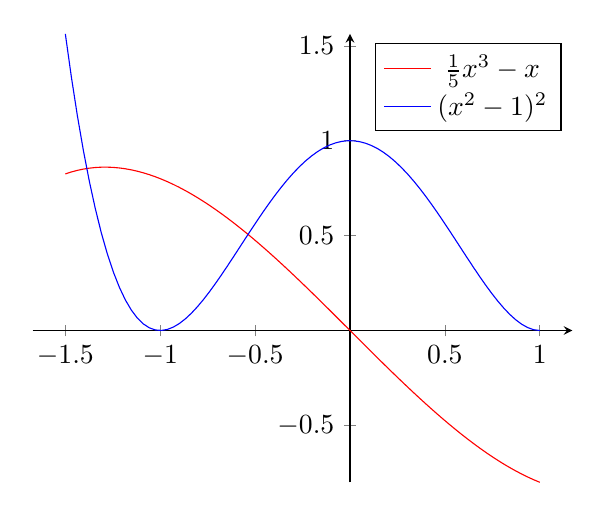
\begin{tikzpicture}
  \begin{axis}[axis lines = center, axis equal,
      domain = -1.5:1,
      legend entries = {$\frac{1}{5}x^3-x$, $(x^2-1)^2$}]
    \addplot[red,samples=80, mark=none] {x^3/5 - x};
    \addplot[blue,samples=80, mark=none] {(x^2-1)^2};
  \end{axis}
\end{tikzpicture}
\end{document}
